[General introduction to discussion]

\section{Performance of Forecasting Models}

 [household energy prediction is unique because of outliers, the same problem is not prominent when predicting for an entire city e.g. future research is (probably) needed to better handle the outlier situation of household prediction, since this topic is underexplored in research]

To investigate the effect of outliers, further analysis and experiments were performed. A maximum monthly consumption threshold of 2000 kWh was selected, due to the majority of observations registering below 2000 kWh, as shown in \autoref{fig:kwh_histogram_2022_2025}. 267 households exceeding this threshold were removed from the sample of 2000 households used for the experiments. The grid search, training, and evaluation process was repeated for each model with the modified data. The resulting scores are found in \autoref{tab:performance-no-outliers}.

The removal of high-consuming households results in a small improvement in MAPE, and large improvements in both RMSE and MAE, confirming that high-consuming households have a great impact on the models' RMSE and MAE performance. The root mean squared errors were roughly half of the original for all models, and mean absolute errors decreased with around y kWh. MAPE scores improved up to 1 percentage point. Notably, the RMSE and MAE scores for the total feature group (both internal and external features) are better than for the internal group when the high-consuming households have been removed. [This suggests that external variables create noise for the households with high consumption, and actually worsen the predictive performance for this group. However, it is clear that the external variables improve the accuracy for households with a lower or medium consumption (vill förtydliga att det troligen bara är de med extremt hög konsumtion som förstör?)]

\begin{table}[H]
    \centering
    \caption{Performance of forecasting models when outlier households (i.e., households with $>$2000 kWh consumption any month) are removed from the data.}
    \label{tab:performance-no-outliers}
    \small
    \begin{tabularx}{\linewidth}{l *{6}{R}}
                       & \multicolumn{3}{c}{\textbf{Internal features}} & \multicolumn{3}{c}{\textbf{Total features}}                                                                                      \\
        \cmidrule(lr){2-4} \cmidrule(lr){5-7}
        \textbf{Model} & \textbf{MAPE (\%)}                             & \textbf{RMSE (kWh)}                         & \textbf{MAE (kWh)} & \textbf{MAPE (\%)} & \textbf{RMSE (kWh)} & \textbf{MAE (kWh)} \\
        \midrule
        RF             & 15.99                                          & 70.67                                       & 38.37              & 15.32              & 69.42               & 37.03              \\
        GBM            & 15.27                                          & 70.41                                       & 37.29              & 14.43              & 66.85               & 35.11              \\
        XGBoost        & 15.25                                          & 70.17                                       & 37.74              & 14.40              & 68.52               & 36.27              \\
        LightGBM       & 15.38                                          & 72.44                                       & 38.52              & 14.37              & 66.47               & 35.30              \\
        CatBoost       & 15.44                                          & 70.03                                       & 37.34              & 15.12              & 66.05               & 35.53              \\
        %(Linear regression) &                                                &                                             &              &               &               &              \\
    \end{tabularx}
\end{table}

\begin{figure}[H]
    \centering
    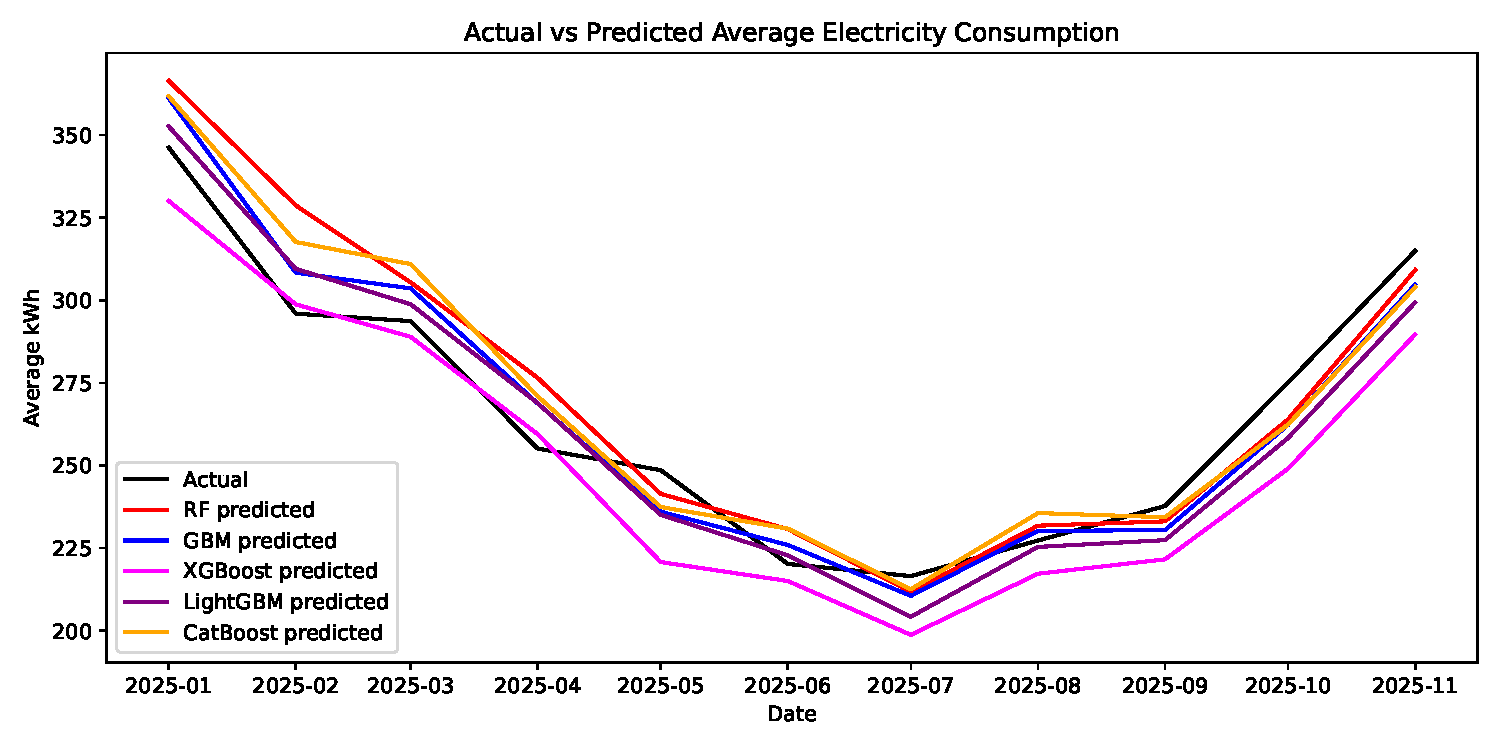
\includegraphics[width=1\linewidth]{figures/avg_predicted_vs_actual_consumption_no_outliers.pdf}
    \caption{.}
    \label{fig:avg-actual-vs-predicted-no-outliers}
\end{figure}

\begin{figure}[H]
    \centering
    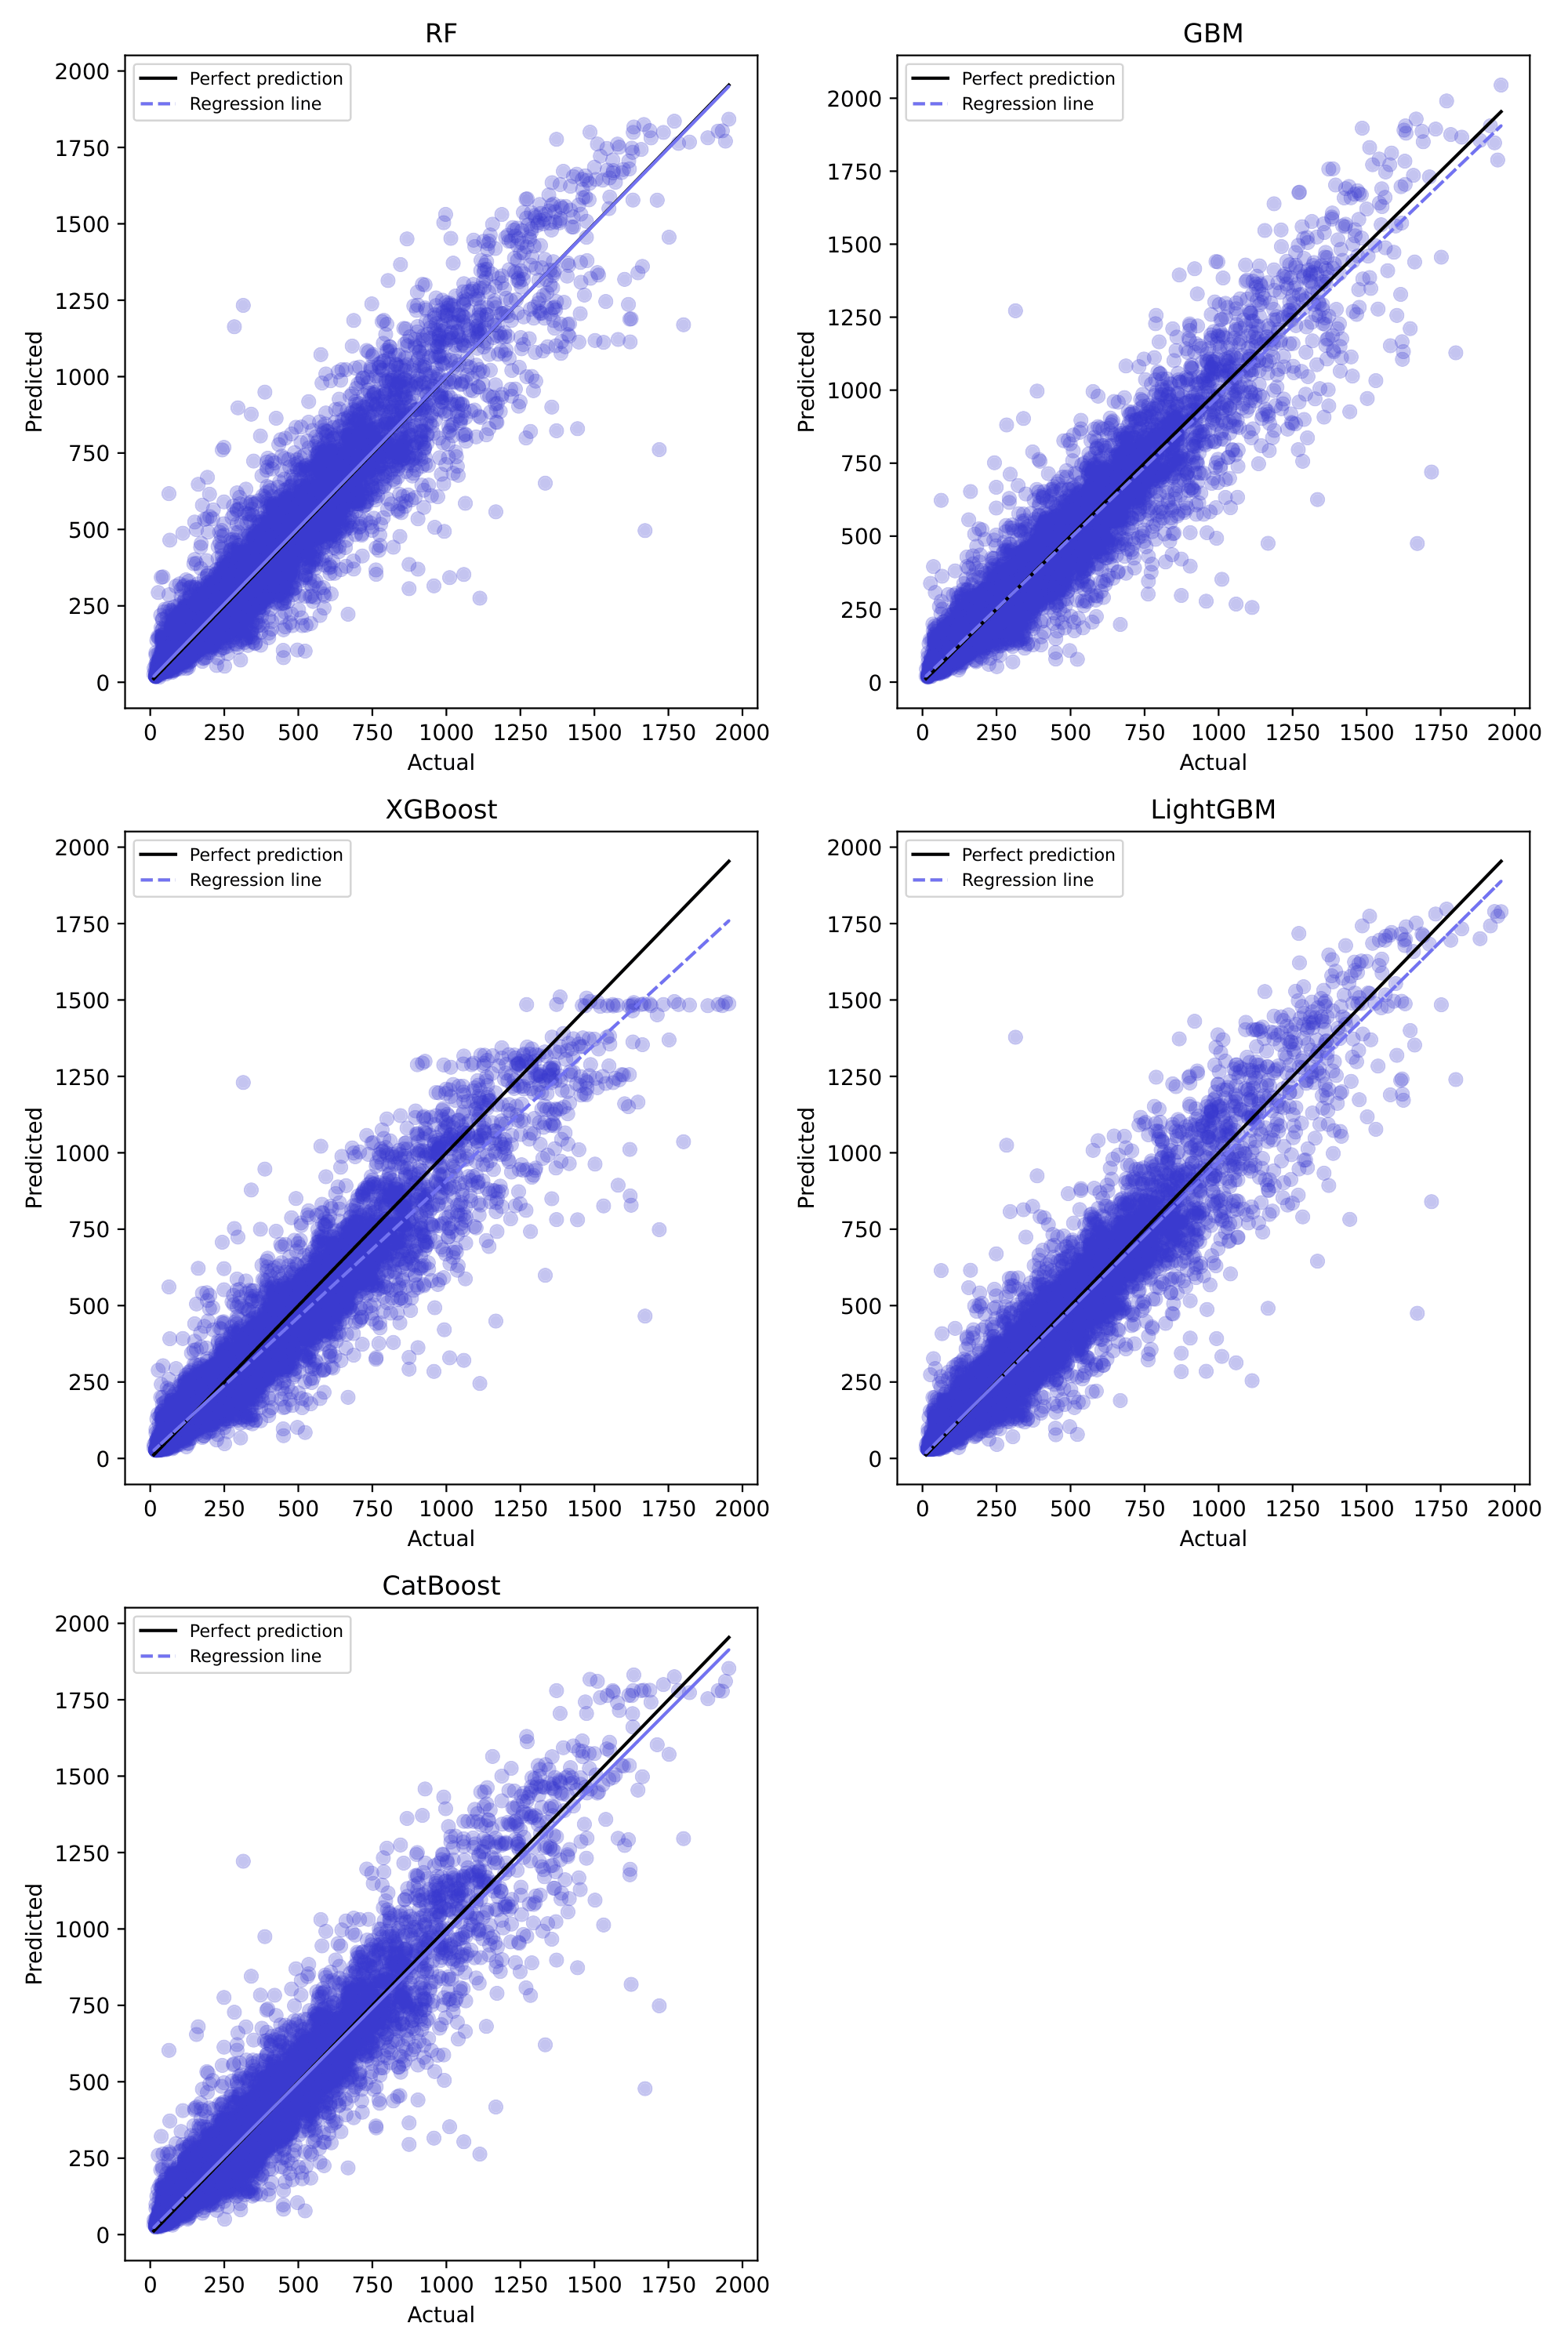
\includegraphics[width=1\linewidth]{figures/scatter_plots_no_outliers.png}
    \caption{.}
    \label{fig:scatter-plots-no-outliers}
\end{figure}

TODO: analysera mer om dessa outliers. alla bör ju ha eluppvärmning tex?

The removed households almost exclusively belonged to the house category (89\%) and vacation home category (10\%), and the majority had electrical heating (70\%).

\section{Explainable AI Forecast Analysis}
 [discuss how SHAP gives better insights than FI, XGBoost example]

The results from the XAI analysis of the forecasts provides insights into the ensemble models' decision-making, as well as perspectives on the methodologies used. A notable observation is that the simple feature importance measure did not always rank the variables' importance in the same way as the more detailed SHAP analysis. For example, the feature importance plot for XGBoost ranked $WCT$ as the most important feature, while the SHAP summary plot showed that several other variables had a more determining impact on the model's predictions.

One pattern evident in all models is that the calendar information had little impact on the forecasts. Previous works have identified holiday indicators as important for electricity consumption forecasting, since consumption patterns change between weekdays and holidays \cite{roman_holidays_2015}. Studies on short-term forecasting highlight holidays as anomalies that need to be handled in a special way, for example by introducing holidays features or by modelling holidays in a special way \cite{moon_advancing_2024,kang_off_2022,trull_one-day-ahead_2021}. However, the results in this experiment indicate that monthly forecasts are not affected by holidays in the same way as the short-term forecasts. This could be due to the effect of holidays smoothing out over the entire month, whereas in the case of e.g. day-ahead forecasting, the entire forecast would be either for a holiday or for a weekday.

    [comparisons with previous works]

\section{Limitations}

 [a big limitation is the insufficient handling of outliers, since there were many. This impacted the model performance greatly. But I just did not know what to do lol]

One limitation with this study is the method of constructing certain features, particularly external ones. All weather variables are aggregated to monthly values using mean. Some weather variables may provide more information using another aggregation method, for example, the monthly total amount of solar radiation may be a better variable than the mean solar radiation. Additionally, the process of aggregating hourly values to a single monthly value can discard valuable information. For example, Lazzari et al. \cite{lazzari_user_2022} found that minimum and maximum temperature were more important than mean temperature, possibly due to minimum and maximum temperatures having a higher variation. This indicates the existence of potential improvements by creating additional features from the weather variables than just the monthly mean. The same potential exists for the construction of more informational holiday indicators. This study only used the simple number of holidays and total number of days per month, while a better indicator could be categorizing months based on holidays.

Another limitation is the grouping of households performed via clustering. The clusters identified via the K-Means method did not show drastically different properties from each other, and the variation in electricity consumption within each cluster was high.
    [clustering was maybe not so successful. Is there a better way to divide the households into consumption groups? And how do we handle outliers in a better way?]

    [the experiments assume that all information is available. This is meant to work in a real-life scenario, where all information might not be available, for example how should new customers be handled? How should the weather data be implemented? Forecasts two weeks ahead exist, but should that be the assumption for the entire month?]